
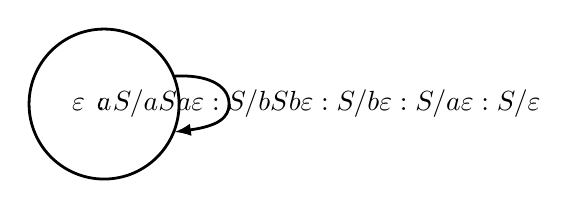
\begin{tikzpicture}[>=latex,line join=bevel,]
  \pgfsetlinewidth{1bp}
%%
\pgfsetcolor{black}
  % Edge: a -> a
  \draw [->] (52.443bp,46.036bp) .. controls (63.028bp,46.728bp) and (72bp,43.383bp)  .. (72bp,36bp) .. controls (72bp,31.155bp) and (68.136bp,28.049bp)  .. (52.443bp,25.964bp);
  \definecolor{strokecol}{rgb}{0.0,0.0,0.0};
  \pgfsetstrokecolor{strokecol}
  \draw (99bp,36bp) node {$\begin{matrix} \varepsilon: S/aSa \\ \varepsilon: S/bSb \\ \varepsilon: S/b \\ \varepsilon: S/a \\ \varepsilon: S/\varepsilon \\ \end{matrix}$};
  % Node: a
\begin{scope}
  \definecolor{strokecol}{rgb}{0.0,0.0,0.0};
  \pgfsetstrokecolor{strokecol}
  \draw (27bp,36bp) ellipse (27bp and 27bp);
  \draw (27bp,36bp) node {$a$};
\end{scope}
%
\end{tikzpicture}

